\chapter{Introduction}  \label{chapter:introduction}
\graphicspath{{introduction/figures/}}

\begin{flushright}
\textit{``More data usually beats better algorithms''}\\
 Anand Rajaraman

\end{flushright}

Business Intelligence (BI) has always been about creating new insight for business by converting data into meaning that can be shared between people to drive change in the organization. One key aspect of creating meaning is to have a common shared understanding of information also known as Semantics.

Classic BI and even the newer Agile Visualization tools focus much of their selling features on attractive and unique visualizations. Preparing data for those visualizations however still remains the far most challenging task in most BI projects large and small. The ultimate goal of BI is to facilitate efficient decisions while eliminating some of the IT headache. Traditionally, BI approaches have been controlled by a centralized version of truth with a wall between IT and the business. Self-service data provisioning aims at removing this wall by providing intuitive dataset discovery, acquisition and integration techniques intuitively to the end user.

\section{Context and Motivation} \label{section:motivation}

Enterprises use a wide range of heterogeneous information systems in their business activities such as Enterprise Resource Planning (ERP), Customer Relationships Management (CRM) and Supply Chain Management (SCM) systems. An enterprise distributed IT landscape contains multiple systems using different technologies and data standards~\cite{Mihindukulasooriya:COLD:13}. In addition to this heterogeneity, the amount of information in enterprise databases and on-line data stores expands exponentially each year. Enterprise Big Data is not big in volume only, but in the associated file formats. The information is also often stored in unstructured and unknown formats.

Data integration is challenging as it requires combining data residing at different sources, and providing the user with a unified view of these data~\cite{Lenzerini:SIGMOD:02}. In large enterprises, it is a time and resource costly task. Various approaches have been introduced to solve this integration challenge. These approaches were primarily based on XML as the data representation syntax, Web Services to provide the data exchange protocols and Service-Oriented Architecture (SOA) as a holistic approach for distributed systems architecture and communication. However, it was found that these technologies are no sufficient to solve the integration problems in large enterprises~\cite{Frischmuth:ISWC:13,Frischmuth:SemWebJorunal:12}. Recently, ontology-based data integration approaches have been suggested where ontologies are used to describe the data, queries and mappings between them~\cite{Wache:IJCAI:01}. A slightly different approach is the use of the Linked Data paradigm~\cite{Bizer:IJSWIS:09} for integrating enterprise data. Enterprises like Google and Microsoft are not only using the Linked Data integration paradigm for their information systems, but are also aiming at building enterprise knowledge bases (like the Google Knowledge Graph powered in part by Freebase\footnote{\url{http://freebase.com}}) that act as a crystallization point for their structured data.

Data becomes more useful when it is open, widely available, in shareable formats and when advanced computing and analysis can yield from it. The quality and amount of structured knowledge available on the web make it now feasible for companies to mine this huge amount of public data and integrate it in their next-generation enterprise information management systems. An example of this external data is the Linked Open Data (LOD) cloud. From 12 datasets cataloged in 2007, it has grown today to nearly 1000 datasets containing more than 82 billion triples\footnote{\url{http://datahub.io/dataset?tags=lod}}~\cite{Bizer:IJSWIS:09}. Data is being published by both the public and private sectors and covers a diverse set of domains from life sciences to media or government data. The LOD cloud is potentially a gold mine for organizations and individuals who are trying to leverage external data sources in order to produce more informed business decisions~\cite{Boyd:Article:11}. This external data can be accessed through public data portals like \texttt{datahub.io} and \texttt{publicdata.eu} or private ones like \texttt{quandl.com} and \texttt{enigma.io}. Analyzing this new type of data within the context of existing enterprise data should bring them new or more accurate business insights and allow better recognition of sales and market opportunities~\cite{LaValle:MIT:11}.

\section{Use Case Scenario}\label{section:scenario}

To enable wide scale and efficient integration of data, there are some efforts needed from various sides. In this thesis, we tackle the issues and challenges from the point of views of two personae:

\begin{itemize}
	\item \textbf{Data Analyst:} A Data Analyst is an experienced professional who is able to collect and acquire data from multiple data sources, filter and clean data, interpret and analyze results and provide ongoing reports.
	\item \textbf{Data Portal Administrator:} A Data Portal Administrator monitors the overall health of a portal. He oversees the creation of users, organizations and datasets. Administrators try to ensure a certain data quality level by continuously checking for spam and manually enhancing dataset descriptions and annotations.
\end{itemize}

Throughout this thesis, we will present a use case scenario involving the two personae to illustrate the challenges and solutions that we provide.

In our scenario, \textbf{Bob} is a Data Analyst working with the Ministry of Transport in France. His favorite tool for crunching, manipulating and visualizing data is SAP Lumira\footnote{\url{http://saplumira.com/}}, a self-service data visualization tool that makes it easy to import data from multiple sources, perform visual BI analysis using intuitive dashboards, interactive maps, charts, and infographics. Bob receives a memo from his management to create a report comparing the number of car accidents that occurred in France for this year, to its counterpart in the United Kingdom (UK). In addition, he is asked to highlight accidents related to illegal consumption of alcohol in both countries.

After examining the ministry's records, Bob is able to collect the data needed to create his report for the French side. Bob also issues an official request to the Department of Transport in UK to collect the data needed. However, Bob knows that the process takes a long time and his management needs the report within days. Bob is familiar with the Open Data movement and starts his journey searching through different data portals in the UK.

\textbf{Mark} is a Data Portal Administrator for the \texttt{data.gov.uk}. He continuously oversees the processes of acquiring, preparing and publishing datasets. Mark always tries to ensure that the data published is of high quality and contains sufficient attached metadata to easily enable search and discovery. Mark often receives complaints about inaccurate or spam datasets. He manually removes and fixes errors while keeping open communication channels with the data-publishing departments.

\section{Research Challenges} \label{section:challenges}

In the scenario presented above, both publishers (Data Portal Administrators) and users (Data Analysts) need pragmatic solutions that help them in their tasks. To enable that, there are some challenging research questions that have to be addressed. These challenges are organized in three main categories as the following:

\subsection{Dataset Integration and Enrichment}

\begin{itemize}
	\item The enterprise heterogeneous data sources raise tremendous challenges. They have inherently different file formats, access protocols or query languages. They possess their own data model with different ways of representing and storing the data. Data across these sources may be noisy (e.g. duplicate or inconsistent), uncertain or semantically similar but yet different. \textbf{Mark} needs powerful tools to map and organize the data in order to have a unified view for these heterogeneous and complex data structures.
	\item Attaching metadata and semantic information to instances can be tricky. An entity is usually not associated with a single generic type in the knowledge base, but rather with a set of specific types which can be relevant or not given the context. \textbf{Mark} is challenged with finding the most relevant entity type within a given context.
	\item Entities play a key role in knowledge bases in general and in the Web of Data in particular. Entities like those in DBpedia, are generally described with a lot of properties. However, it is difficult for \textbf{Bob} to assess which ones are more ``important'' than others for particular tasks such data augmentation and visualizing the key facts of an entity.
	\item Social networks are not just gathering Internet users into groups of common interests, they are also helping people follow breaking news, contribute to online debates or learn from others. They are transforming Web usage in terms of users' initial entry point, search, browsing and purchasing behavior. However, integrating information from these social networks can be tricky to \textbf{Mark} due to the vast amount of data available which makes hard to spot what is relevant in a timely manner.
\end{itemize}

\subsection{Dataset Maintenance \& Discovery}

\begin{itemize}
	\item Even though popular datasets like DBPedia\footnote{\url{http://dbpedia.org}} and Freebase are well known and widely used, there are other hidden useful datasets not being used. Indeed these datasets may be useful for specialized domains, however without proper registry of topics, it is difficult for data analysts like \textbf{Bob} to find them~\cite{Lalithsena:WI:13}.
	\item The growing amount of data requires rich metadata in order to reach its full potential. This metadata enables dataset discovery, understanding, integration and maintenance. Despite the various models and vocabularies describing datasets metadata, the ability to have an overview of the dataset by inspecting its metadata can be limited. For example, \textbf{Bob} has difficulties finding datasets with a specific geographical coverage as this information is missing from almost all of the examined datasets profiles.
	\item Users, organizations and governments are empowered to publish datasets. However, data portal administrators like \textbf{Mark} need to continuously and manually check portals to detect Spam and maintain high quality data.
\end{itemize}

\subsection{Dataset Quality}

Linked Data consists of structured information supported by models, ontologies and vocabularies and contains query endpoints and links. This makes data quality assurance a challenge. Despite the fact that Linked Open Data quality is a trending and highly demanded topic, very few efforts are currently trying to standardize, track and formalize frameworks to issue scores or certificates that will help data consumers in their integration tasks. Data portal administrators like \textbf{Mark} need to have an overall view of their portals quality and want to incorporate such metrics in the existing dataset profiles. On the other hand, data analysts and users like \textbf{Bob} want to know beforehand if the dataset on hand is of a certain degree of quality to be used in their reports.

\section{Thesis Contributions} \label{section:contribution}

In this thesis, we propose a framework (see Figure~\ref{fig:architecutre_diagram}) to enable self-service data provisioning for internal and external data sources in the enterprise. The framework contributes to the three main challenges described above. In summary, the main contributions of this work are as follows:

\begin{figure}[!ht]
  \centering
  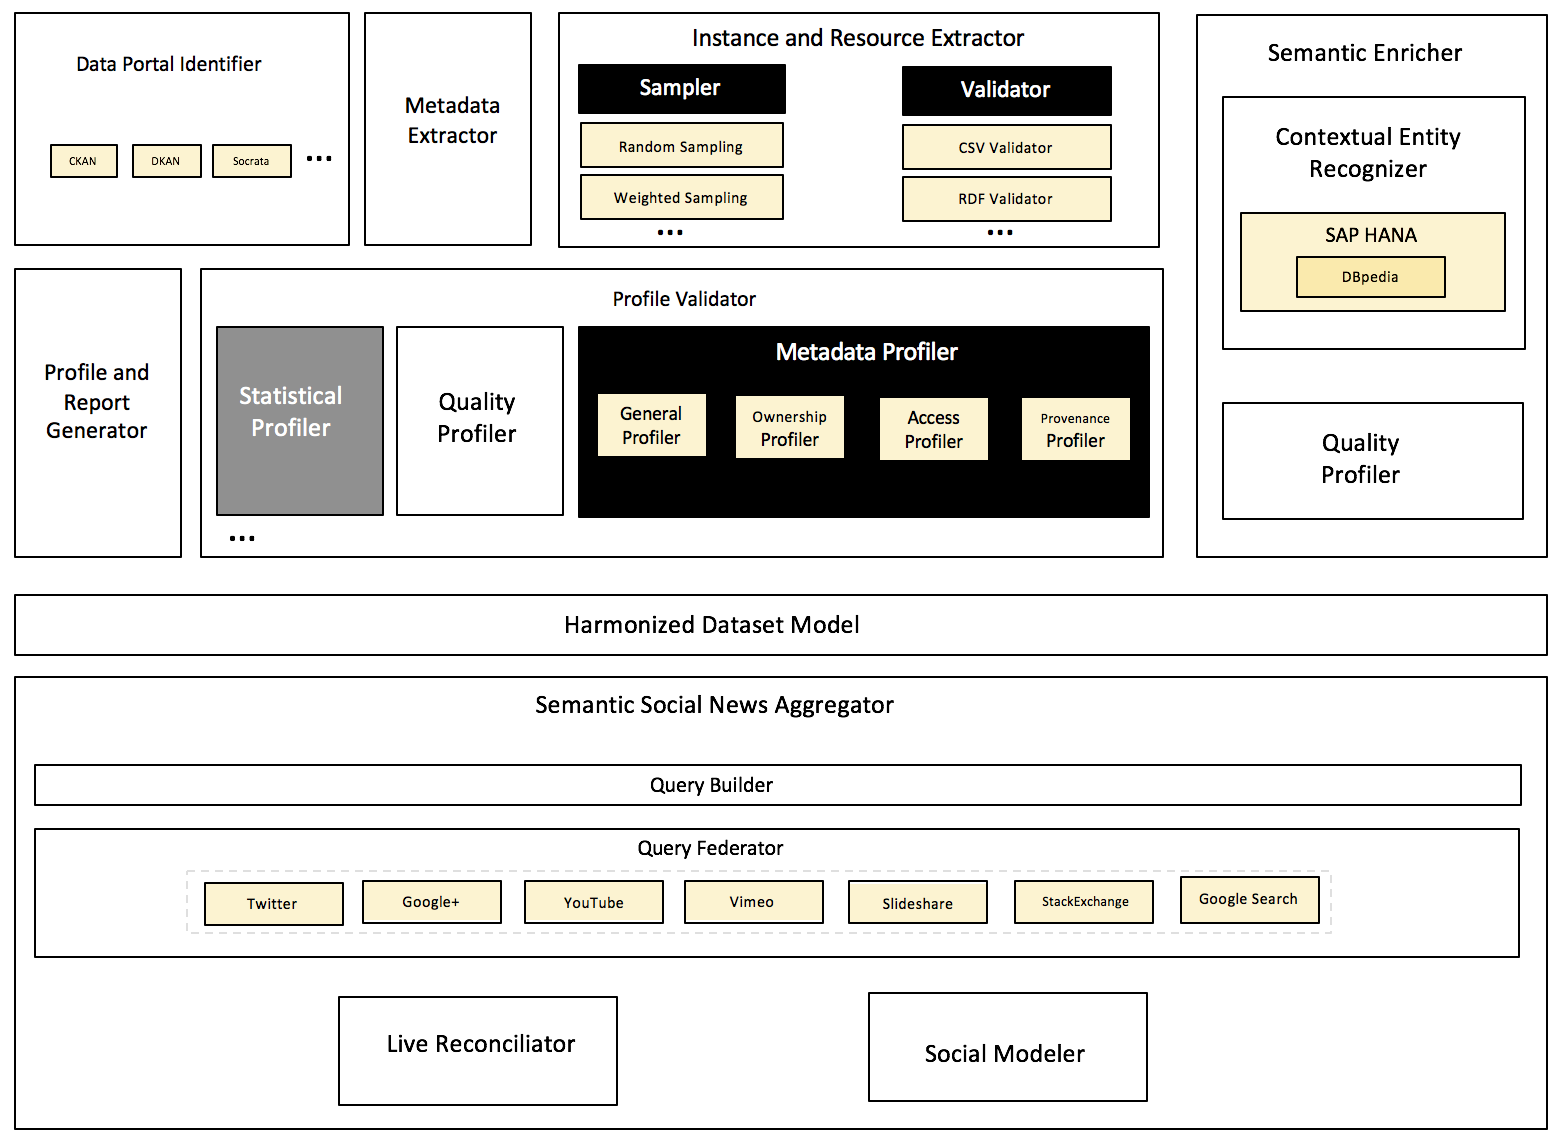
\includegraphics[scale=0.5]{architecutre_diagram.png}
  \caption{Architecture diagram for enabling self-service data provisioning}
  \label{fig:architecutre_diagram}
\end{figure}

\subsection{Contributions on Dataset Maintenance \& Discovery}

Regarding this aspect of our research, we have achieved the following tasks:
\begin{itemize}
	\item We surveyed the landscape of various models and vocabularies that describe datasets on the web. Since establishing a common vocabulary or model is the key to communication, we identified the need for an harmonized dataset metadata model containing sufficient information so that consumers can easily understand and process datasets (see Section~\ref{section:datasetModels}). First, we implemented a set of mappings between each properties of the surveyed models. This has lead to the design of HDL, a harmonized dataset model, that takes the best out of these models and extends them to ensure complete metadata coverage to enable data discovery, exploration and reuse (see Section~\ref{section:hdl}).
	\item We have analyzed the landscape of dataset profiling tools and discovered various gaps (see Section~\ref{section:roomba-related-work}). As a result, we proposed Roomba, a scalable automatic framework for extracting, validating, correcting and generating descriptive linked dataset profiles (see Section~\ref{section:roomba-framework}). Roomba applies several techniques in order to check the validity of the metadata provided and to generate descriptive and statistical information for a particular dataset or for an entire data portal.
\end{itemize}

\subsection{Contributions on Dataset Quality Control}
Concerning our contributions on Linked Data quality assessment, we have achieved the following tasks:
\begin{itemize}
	\item We proposed a linked data quality assessment framework focusing on the data's objective metrics. We have identified a total of 64 quality indicators that were mapped when suitable to four main categories (entity, dataset, links, models) corresponding to the core Linked Data publishing principles. (see Section~\ref{section:data-quality-classification}).
	\item Upon surveying the landscape of data quality tools, we noticed a lack in automatic tools to check the dataset quality metrics proposed in our framework (see Section~\ref{section:quality-tools}). As a result, we extended Roomba to perform a set of data quality checks on Linked datasets. Our extension covers most of the quality indicators proposed with focus on completeness, correctness, provenance and licensing (see Section~\ref{section:quality-assessment-framework}).
\end{itemize}

\subsection{Contributions on Dataset Integration and Enrichment}

Regarding this aspect of our research, we have achieved the following tasks:
\begin{itemize}
	\item We created a framework called RUBIX that enables mashing-up potentially noisy enterprise data and external data. The framework leverages reference knowledge bases to annotate data with a set of semantic concepts (metadata). One of the advantages of this metadata is to enhance the matching process of heterogeneous data sources within an enterprise (see Section~\ref{Section:RUBIX}).
	\item The metadata attached by RUBIX can be further used to enrich existing datasets. However, concepts are often represented with a large set of properties. To better recommend the top ``important'' properties for a concept, we reversed engineer the choices made by Google when creating knowledge graph panels and presented these choices explicitly using the Fresnel vocabulary, so that any application could read this configuration file for deciding which properties of an entity is worth to enrich (see Section~\ref{Section:EKG}).
	\item Aggregating relevant social news is not an easy task. We provide an Application Programming Interface (API) that enables semantic social news aggregation called SNARC. We designed a sample frontend application leveraging SNARC's capabilities to enable users to discover relevant social news instantly (see Chapter~\ref{chapter:snarc}.
\end{itemize}

\section{Thesis Outline} \label{section:outline}
The work presented in this thesis first describes a standard model to represent dataset profiles. Then it focuses on techniques to automatically generate and validate these profiles.

The rest of this manuscript is composed of two major parts:

In part~\ref{part:dataset_profiling}, we focus on the development of a framework that automatically validates and generates dataset profiles. We highlight the extensibility of this framework and show the results of running it across various data portals. The contributions of this part have been published in ~\cite{Assaf:DQMST:12,Assaf:WWW:15,Assaf:IJSWIS:15,Assaf:PROFILES:15,Assaf:ESWC:PROFILES:15,Assaf:ESWC:LDQ:15}.

\begin{itemize}
  \item \textbf{Chapter~\ref{chapter:part1-background}} overviews the background of our work in data profiling and quality assurance. We first introduce the basic concepts in the Semantic Web and the important aspects related to (Linked) Open Data. Then, we describe the concepts of data profiling and data quality.
	\item \textbf{Chapter~\ref{chapter:hdl}} conducts a unique and comprehensive survey of seven metadata models: CKAN, DKAN, Public Open Data, Socrata, VoID, DCAT and Schema.org. We propose a Harmonized Dataset modeL (HDL) based on this survey. We describe use cases that show the benefits of providing rich metadata to enable dataset discovery and search and spam detection.
	\item \textbf{Chapter~\ref{chapter:roomba}} emphasizes the need for tools that are able to identify various issues in this metadata and correct them automatically. We introduce Roomba, a scalable automatic approach for extracting, validating, correcting and generating descriptive linked dataset profiles. Afterwards, we present the results of running our framework on prominent data portals and analyze the results. We show that the overall state of Linked Data portals needs more attention.
	\item \textbf{Chapter~\ref{chapter:data-quality}} surveys the landscape of Linked Data quality tools and build upon previous efforts with focus on objective data quality measures. We further present a comprehensive objective quality framework applied to the Linked Open Data. We identify several gaps in the current tools and find the need for a comprehensive evaluation and assessment framework for measuring quality on the dataset level. We extend Roomba to calculate 82\% of the suggested datasets objective quality indicators.
\end{itemize}

In part~\ref{part:data_integration}, we focus on the challenges of external data integration in the enterprise. We focus on the development of a semantic enrichment framework and show the advantages of such enrichments in enhancing schema matching results and data enrichment.The contributions of this part have been published in ~\cite{Assaf:WOD:12,Assaf:ESWC:13}

\begin{itemize}
  \item \textbf{Chapter~\ref{chapter:part2-background}} overviews the background of our work in data integration and enrichment. We introduce the basic concepts in Business Intelligence and Data Warehousing and describe the various technologies and systems in SAP's ecosystem.
	\item \textbf{Chapter~\ref{chapter:rubix}} presents a framework that enables business users to semi-automatically combine potentially noisy data residing in heterogeneous silos. Semantically related data is identified and appropriate mappings are suggested to users. We also show that it is possible to reveal what are the ``important'' properties of entities by reverse engineering the choices made by Google when creating knowledge graph panels and by comparing users preferences obtained from a user survey.
	\item \textbf{Chapter~\ref{chapter:snarc}} emphasizes the need for tools that are able to aggregate relevant social news to a certain context. We introduce SNARC, a semantic social news aggregation framework that leverages live rich data that social networks provide to build an interactive rich experience on the Internet.
\end{itemize}